\section{The basics of Quantum Monte-Carlo}

\subsection{The basic idea}

\begin{frame}
 Using the \textit{projection operator} $\OP{P}(\tau)$ on an arbitrary state $\ket{\Psi_T}$ projects the state onto the ground state of $\OP{H}$ as $\tau\to\infty$.  
 \pause
  \begin{align*}
   \onslide<2->{\OP{P}(\tau)\ket{\Psi_T} &= \exp(-(\OP{H} - E_0)\tau)\ket{\Psi_T} \\}
   \onslide<3->{&= \exp(-(\OP{H} - E_0)\tau)\sum_{k} C_k\ket{\Psi_k} \\}
   \onslide<4->{&= \sum_{k} C_k\exp(-(E_k - E_0)\tau) \ket{\Psi_k} \\}
   \onslide<5->{&= C_0\ket{\Psi_0} + \sum_{k=1} C_k\exp(-\Delta E_k\tau) \ket{\Psi_k},}
  \end{align*}

  \onslide<5->where $\Delta E_k > 0$ and $C_k = \braket{\Psi_k}{\Psi_T}$. 

\end{frame}

\begin{frame}
 In other words
 
 \begin{equation}
  \lim_{\tau\to\infty}\bra{\mathbf{r}}\OP{P}(\tau)\ket{\Psi_T} = \braket{\Psi_0}{\Psi_T}\Psi_0(\mathbf{r}).
 \end{equation}

 \pause
 \textbf{Idea I}: Use an arbitrary \textit{trial wave function} $\Psi_T(\mathbf{r})$ and perform the projection.
 
 \pause
 \vspace{0.5cm}
 \textbf{Problem}: Requires a priori knowledge of the exact ground state energy $E_0$.
 
 \pause
 \vspace{0.5cm}
 \textbf{Solution}: Introduce a \textit{trial energy} $E_T(\tau)$. Will work as long as the trial energy drops below $E_1$ at a certain stage (and stays there). 
 
\end{frame}

\begin{frame}
 
 In order to relate the projection process to a \textit{Markow chain} Monte-Carlo process, $\tau$ needs to be split into sequential steps $\delta\tau$. 
 \pause
 \vspace{0.5cm}
 
 This is achieved by using the following property of the projection operator
 
 \begin{align*}
  \OP{P}(\tau + \delta\tau) &= \exp(-(\OP{H} - E_T(\tau + \delta\tau))(\tau + \delta\tau)) \\
                            &=  \exp(-(\OP{H} - E_T(\tau + \delta\tau))\delta\tau) \\
                            & \qquad \times\exp(-(\OP{H} - E_T(\tau + \delta\tau))\tau) \\
                            &\simeq \exp(-(\OP{H} - E_T(\tau + \delta\tau))\delta\tau)\OP{P}(\tau),
 \end{align*}

where the relation is approximate due to $E_T$ not being constant.
 
 
 
\end{frame}

\begin{frame}
  Let $\ket{\Phi(\tau)}$ represent $\OP{P}(\tau)\ket{\Psi_T}$. Using the relation from the previous slide reveals
  \pause
  \begin{align*}
   \onslide<2->{\Phi(\mathbf{r}, \tau + \delta\tau) &= \braket{\mathbf{r}}{\Phi(\tau + \delta\tau)} \\ &= \bra{\mathbf{r}}\OP{P}(\tau + \delta\tau)\ket{\Psi_T} \\}
   \onslide<3->{&\simeq  \bra{\mathbf{r}}\exp(-(\OP{H} - E_T)\delta\tau)\OP{P}(\tau)\ket{\Psi_T} \\}
   \onslide<4->{&=\bra{\mathbf{r}}\exp(-(\OP{H} - E_T)\delta\tau)\ket{\Phi(\tau)}  \\}
   \onslide<5->{&= \int_\mathbf{r'}\bra{\mathbf{r}}\exp(-(\OP{H} - E_T)\delta\tau)\ket{\mathbf{r'}}\Phi(\mathbf{r'}, \tau)\mathrm{d}\mathbf{r'},}
  \end{align*}
  
  \pause\pause\pause\pause
  where $\bra{\mathbf{r}}\exp(-(\OP{H} - E_T)\delta\tau)\ket{\mathbf{r'}} \equiv G(\mathbf{r'}, \mathbf{r}; \delta\tau)$ is a \textit{Green's function} interpreted as the transition probability between $\mathbf{r}$ and $\mathbf{r'}$.
    
\end{frame}

\begin{frame}
 \textbf{Idea}: In order to relate the Green's function to well known Markow processes, the exponential is split
 
 \begin{align*}
  \exp(-(\OP{H} - E_T)\delta\tau) &= \exp\left(\frac{1}{2}\nabla^2\delta\tau - (\OP{V} - E_T)\delta\tau\right)\\
     &= \exp\left(\frac{1}{2}\nabla^2\delta\tau\right)\exp( - (\OP{V} - E_T)\delta\tau) \\
     & \qquad  + \mathcal{O}(\delta\tau^2),
 \end{align*}
 
 where the kinetic part describes a diffusion process with diffusion constant $D=\frac{1}{2}$, and the potential part desribes a weighting (linear in position space). This is referred to as the \textit{short time approximation}.

 
\end{frame}

\begin{frame}
 \textbf{Problem}: The Green's function has singular points in the Coulomb interaction.
 \vspace{0.5cm}
 
 \pause
 
 \textbf{Solution}: By evolving $f(\mathbf{r}, \tau) = \Phi(\mathbf{r}, \tau)\Psi_T(\mathbf{r})$ instead of $\Phi(\mathbf{r}, \tau)$ alone, the singularities are \emph{implicitly} taken care of.
  
 \end{frame}

 \begin{frame}
   Originally:
 \begin{equation*}
  \frac{\partial \Phi(\mathbf{r}, \tau)}{\partial\tau} = \left[\frac{1}{2}\nabla^2 - \left(\OP{V} - E_T\right)\right]\Phi(\mathbf{r}, \tau).
 \end{equation*}
 
 \pause
 
 \textit{Importance sampled}:
  \begin{equation}
  \frac{\partial f(\mathbf{r}, \tau)}{\partial\tau} = \left[\frac{1}{2}\nabla\cdot\left(\nabla - \mathbf{F}(\mathbf{r})\right) - (E_L(\mathbf{r}) - E_T)\right]f(\mathbf{r}, \tau),
 \end{equation}
 
 where
 
\begin{equation}
  \mathbf{F}(\mathbf{r}) =  2\Psi_T(\mathbf{r})^{-1}\nabla \Psi_T(\mathbf{r})
\end{equation}

is the \textit{quantum force} and 

\begin{equation} 
E_L(\mathbf{r}) = \Psi_T(\mathbf{r})^{-1}\OP{H}\Psi_T(\mathbf{r})
\end{equation}

is the \textit{local energy}. 

\end{frame}

\begin{frame}
 The Green's functions have closed form solutions on the form
 
 \begin{align*}
  G_{\mathrm{Diff}}(\mathbf{r}', \mathbf{r}; \delta\tau) &\propto \exp\left(-\left|\mathbf{r}-\mathbf{r}' - D\delta\tau \mathbf{F}(\mathbf{r})\right|^2/4D\delta\tau\right), \\
  G_{\mathrm{B}}(\mathbf{r}', \mathbf{r}; \delta\tau) &\propto \exp\left(-\left(\frac{1}{2}\left[E_L(\mathbf{r}) + E_L(\mathbf{r}')\right] - E_T\right)\delta\tau\right),
 \end{align*}

 where $\mathrm{B}$ denotes \textit{branching}.
 
\end{frame}

\begin{frame}
 The process of projection is modelled by letting an ensemble of walkers span $f(\mathbf{r}, \tau)$. An iteration involves diffusing all the walkers and distributing new weights. 
\end{frame}

\begin{frame}
\frametitle{Branching}

\textbf{Idea}: The weights are modelled by spawning and killing walkers with a rate equal to $G_\mathrm{B}$. 

\pause
\vspace{0.5cm}
\textbf{Problem}: $G_\mathrm{B}$ is not necessarily an integer.

\pause
\vspace{0.5cm}
\textbf{Solution}: Create $\mathrm{floor}(G_\mathrm{B})$ copies with a $G_\mathrm{B} - \mathrm{floor}(G_\mathrm{B})$ chance of creating an additional copy.

\vspace{0.5cm}
\pause
Or more compact: Create 

\begin{equation}
\overline{G}_\mathrm{B} = \mathrm{floor}(G_\mathrm{B} + a)
\end{equation}

copies, where $a \in [0,\,1)$ is a uniformly distributed random number. If the value is zero, the walker dies.

\end{frame}


\begin{frame}
\frametitle{Branching}

\begin{figure}
\begin{center}
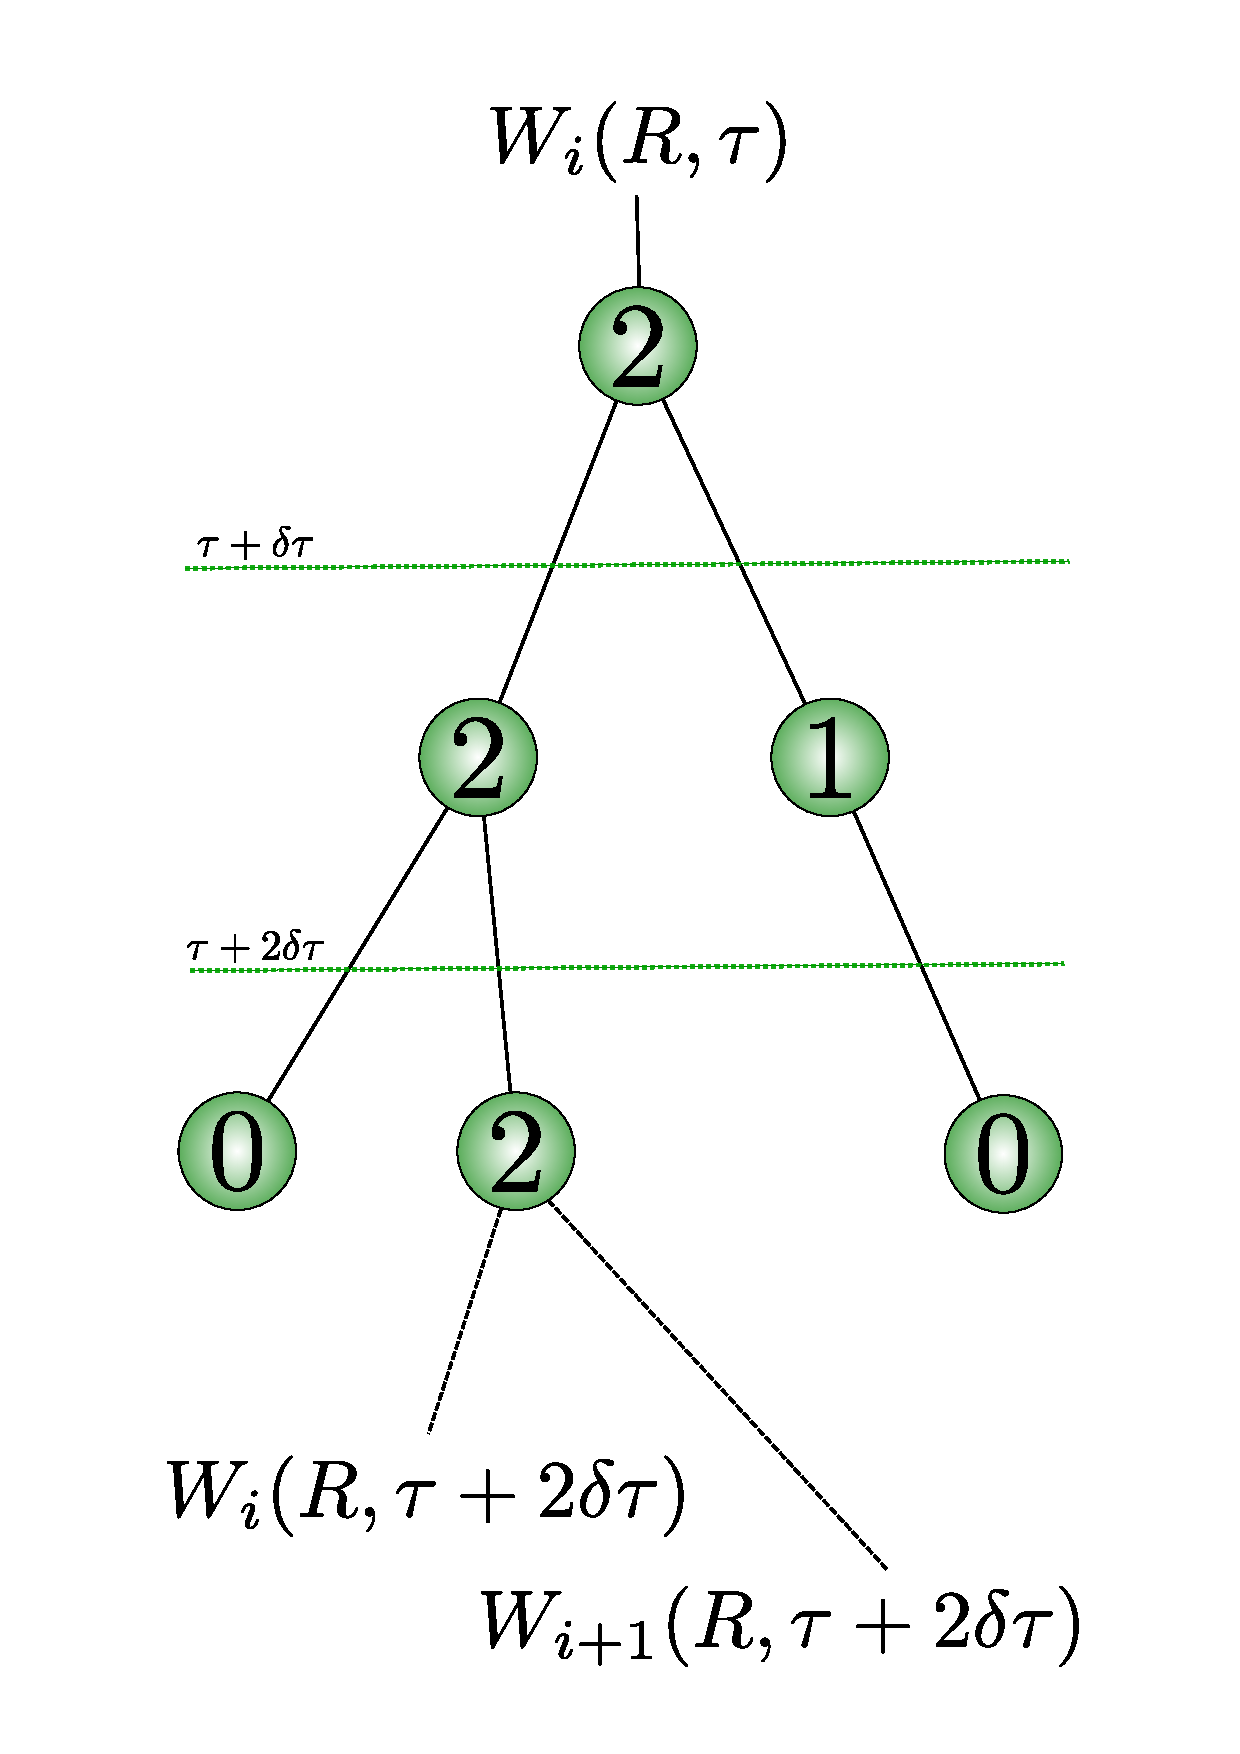
\includegraphics[scale=0.2]{../graphics/branching.pdf}
\end{center}
\caption{Branching illustrated. The integer values represent $\overline{G}_\mathrm{B}$.}
\end{figure}

\end{frame}

\begin{frame}
 \frametitle{Diffusion}
 
 The diffusion equation representing $G_\mathrm{Diff}$ is the so-called \textit{Fokker-Planch equation}. 
 
 \pause
 \vspace{0.5cm}
 
 Anisotropic diffusion process. The quantum force pushes the walkers into regions of higher probability. 
 
 \pause
 \vspace{0.5cm}
 
 According to the Fokker-Planch formalism, a new position $\mathbf{r}_{i+1}$ is calculated from the old one, $\mathbf{r}_i$, as follows
 
 \begin{equation}
  \mathbf{r}_{i+1} = \mathbf{r}_i + D\delta\tau\mathbf{F}(\mathbf{r}_i) + \mathbf{\xi}, 
 \end{equation}

where $\mathbf{\xi}$ is a vector of normal distributed random numbers with variance $\sqrt{2D\delta\tau}$.
 
\end{frame}

\begin{frame}
\frametitle{Diffusion}

\textbf{Problem}: Due to a finite time step, the previous equations do not guarantee convergence.  

\pause
\vspace{0.5cm}

\textbf{Solution}: The \textit{Metropolis algorithm} will correct this bias:  

\begin{equation}
  A(i\,\rightarrow\,j) = \min\{R_G(i\,\rightarrow\,j)R_\psi(i\,\rightarrow\,j)^2, \,1\},
\end{equation}

where $i\,\rightarrow\,j$ denotes a transition from state $i$ to state $j$, $A$ is the probability of accepting the transition, 

\begin{equation*}
 R_G(i\,\rightarrow\,j) = G_\mathrm{diff}(\mathbf{r}_{i}, \mathbf{r}_{j}; \delta\tau)/G_\mathrm{diff}(\mathbf{r}_{j}, \mathbf{r}_{i}; \delta\tau),
\end{equation*}

and

\begin{equation*}
 R_\psi(i\,\rightarrow\,j) = |\Psi_T(\mathbf{r}_i)/\Psi_T(\mathbf{r}_j)|.
\end{equation*}

\end{frame}


%% 15


\begin{frame}
 Fixed node approximation
\end{frame}

\begin{frame}
 variational principle.
 VMC
\end{frame}

\begin{frame}
also variational. A bit more tricky to show.
 DMC
\end{frame}

\begin{frame}
 Selecting the trial wave function.
 Choose a Slater determinant of similar eigenstates.
\end{frame}

\begin{frame}
 Introduce alpha
\end{frame}


\begin{frame}
 Jastrow. 
\end{frame}

\begin{frame}
 select opt var par by finding energy minimum.
\end{frame}





















% \begin{frame}
% \frametitle{Diffusion}
% 
% Starting from the condition of \textit{detailed balance}
% 
% ...
% 
% \end{frame}

 














\begin{frame}
 End of section.
\end{frame}
